\documentclass[../Main/main.tex]{subfiles}

\begin{document}
	\graphicspath{{../Time dependent equations/figs/}}
	\chapter{Convergence of Richards' equation}
	In this chapter we use the results from chapter three to prove convergence of the Richards equation discretized in space with MPFA-L method, in time with backward Euler and linearized with the L-scheme.
	We start by considering the Richards' equation without the gravity term in an isotropic medium: Find $\psi = \psi(x,t)$ such that
	\begin{equation}\label{eq:richards w bc}
		\left \{
		\begin{aligned}[c]
			\partial_t \theta(\psi) - \nabla \cdot \left (\kappa(\theta (\psi)) \nabla \psi \right ) &= f, \\
			\psi &= 0, \\
			-\kappa(\theta (\psi)) \nabla \psi &= g_N,\\
			\psi &= u_0,
		\end{aligned}
		\ \ \
		\begin{aligned}[c]
			\text{ in }& \Omega \times (0,T]\\
			\text{ on }& \partial \Gamma_D \times (0,T]\\
			\text{ on }& \partial \Gamma_N \times (0,T)\\
			\text{ on }& \Omega \times \left\{t=0\right \}
		\end{aligned}
		\right.
	\end{equation}
	This equation has a non linearity in the flux, $\bm{q}=-\kappa(\theta (\psi)) \nabla \psi$, which makes it hard to apply our results, as they require a homogeneous medium. The hydraulic conductivity, $\kappa(\theta (\psi))$, depends on our solution which is heterogeneous, and is thus itself heterogeneous.
	To remedy this we use the Kirchhoff transform 
	\begin{equation}
		\begin{aligned}
			\mathcal{K} :\mathbb{R} &\rightarrow \mathbb{R}^{+}\\
			\psi &\mapsto \int_{0}^{\psi} \kappa(\theta(\phi)) \ d \phi = u.
		\end{aligned}
	\end{equation}
	As previously discussed, the functions $\theta(\cdot)$ and $\kappa(\cdot)$ are continuous, monotone increasing functions, the Kirchhoff transform, $\mathcal{K}$, therefore has an inverse, $\mathcal{K}^{-1}$. 
	We define
	\begin{equation}
		\begin{aligned}
			b(u) &:= \theta(\mathcal{K}^{-1}(u))\\
			k(u) &:= \kappa (\theta (\mathcal{K}^{-1}(u))).
		\end{aligned}
	\end{equation}
	\todo[inline]{make assumptions ensuring that b is nicely behaved}
	by the chain rule, we get
	\begin{equation}
		\nabla u = \kappa(\theta(\psi))\nabla \psi.
	\end{equation}
	We can write the Richards' equation \eqref{eq:richards w bc} in the transformed variable $u$ to get: Find $u=u(x,t)$ such that 
	\begin{equation}\label{eq:richards simple}
	\left \{
	\begin{aligned}[c]
		\partial_t b(u) - \nabla \cdot \nabla u &= f, \\
		u &= 0, \\
		-\nabla u &= g_N,\\
		u &= u_0,
	\end{aligned}
	\ \ \
	\begin{aligned}[c]
		\text{ in }& \Omega \times (0,T]\\
		\text{ on }& \partial \Gamma_D \times (0,T]\\
		\text{ on }& \partial \Gamma_N \times (0,T)\\
		\text{ on }& \Omega \times \left\{t=0\right \}
	\end{aligned}
	\right.
\end{equation}
We start by discretizing \eqref{eq:richards simple} with the MPFA-L method, we divide our domain into $d$ quadrilaterals (control volumes). Writing \eqref{eq:semidiscrete FVM} in vector form we find $\tilde{u}_h \in \mathbb{R}^d$ such that:
	\begin{equation}
		\partial_t\pmb{B}^{V} b(\tilde{u}_h) + \pmb{A}^V \tilde{u}_h = \pmb{q}^V. 
	\end{equation}
	We can then discretize in time using backward euler. Given $ \tilde{u}_h^{n-1},\pmb{q}^n \in \mathbb{R}^d$ we should then find $ \tilde{u}_h^n \in \mathbb{R}^d$ such that: 
	\begin{equation} \label{eq:non-linear richards FVM}
		\pmb{B}^V  b(\tilde{u}_h)^n + \tau \pmb{A}^V \tilde{u}_h^n = \tau \pmb{q}^{Vn} + \pmb{B}^V  b(\tilde{u}_h)^{n-1}.
	\end{equation}
	Now we need to linearize \eqref{eq:non-linear richards FVM} with the L-scheme. We see from \eqref{eq:L-scheme} that the applying this linearization leads to the equation:
	\begin{equation}\label{eq:linearized richards fvm}
		L\pmb{B}^V(\tilde{u}^{n,j}_h-\tilde{u}^{n,j-1}_h) + \tau \pmb{A} \tilde{u}_h^{n,j} = -\pmb{B}^V \theta (\tilde{u}_h^{n,j-1})  + \tau \pmb{q}^{Vn} +  \pmb{B}^V \theta (\tilde{u}_h^{n-1}).
	\end{equation}
	The above equation can be solved for $\tilde{u}_h^{n,j}$, and is in principal the same as solving a time discretized heat equation \eqref{eq:stationary_heat}, which we have proved equivalence with the modified finite element method for.\par
	Let us see how it would look if we discretized \eqref{eq:richards simple} with the modified finite element method. Let $u_h, v_h\in V_h$, where $V_h$ is defined as piecewise linear functions as in definition \ref{def:linear ansatz}. Then our semidisrectization would be to find $u_h \in V_h$ such that
	\begin{equation}
		\left \langle \partial_t\hat{I}_h b(u_h^n),\hat{I}_h v_h \right \rangle_0 + \left \langle \nabla u^n_h, \nabla v_h \right \rangle_0 = \left \langle q,v_h \right \rangle_0 \ \ \forall v_h \in V_h.
	\end{equation}
	Next we would discretize in time, our discretization now reads; given $u_h^{n-1} \in V_h$ find $u_h \in V_h$
	\begin{equation}
		\left \langle \hat{I}_h b(u_h^n),\hat{I}_h v_h \right \rangle_0 +\tau \left \langle  \nabla u^n_h, \nabla v_h \right \rangle_0 = \tau \left \langle q^n,\hat{I}_h v_h \right \rangle_0 + \left \langle \hat{I}_h b(u_h^{n-1}),\hat{I}_h v_h \right \rangle_0
	\end{equation}
	for all $v_h \in V_h$. Finally we also linearize this with the L-scheme. Following the same procedure as for \eqref{eq:linearized richards fvm} we get; given  $u_h^{n-1},u_h^{n,j-1} \in V_h$ find $u_h^{n,j} \in V_h$ such that
	\begin{equation}\label{eq:linearized richards fem}
		\begin{aligned}
			&L \left \langle \hat{I}_h u^{n,j}_h -  \hat{I}_h u^{n,j-1}_h,\hat{I}_h v_h \right \rangle_0 + \tau \left \langle  \nabla u^{n,j}_h,\nabla v_h \right \rangle \\&=\tau \left \langle q^n,\hat{I}_h v_h \right \rangle_0 + \left \langle \hat{I}_h u_h^{n-1},\hat{I}_h v_h \right \rangle_0 -\left \langle \hat{I}_h b(u^{n,j-1}_h),\hat{I}_h v_h \right \rangle_0
		\end{aligned}
	\end{equation}
	for all $v_h \in V_h$. Since the mass matrix is diagonal with our modified finite element method, we can express \eqref{eq:linearized richards fem} as a matrix-vector equation similar to the MPFA-L method \eqref{eq:linearized richards fvm}.  Let $\hat{u}_h^{n,j} \in \mathbb{R}^d$ be the coefficients that together with the basis functions that represents $u_h^{n,j} \in V_h$. Then our \eqref{eq:richards simple} discretized with modified finite elements in space, backward euler in time and L-scheme linearization reads; given $\hat{u}_h^{n,j-1},\hat{u}_h^{n-1} \in \mathbb{R}^d$ find  $\hat{u}_h^{n,j} \in \mathbb{R}^d$ such that 
	\begin{equation}\label{eq:linearized richards fem system}
		L\pmb{B}(\hat{u}^{n,j}_h-\hat{u}^{n,j-1}_h) + \tau \pmb{A} \hat{u}_h^{n,j} = -\pmb{B} \theta (\hat{u}_h^{n,j-1})  + \tau \pmb{q}^n +  \pmb{B} b (\hat{u}_h^{n-1}).
	\end{equation}
	We can now state an important result for obtaining a convergence estimate for Richards' equation.
	\begin{lemma}
		The system \eqref{eq:linearized richards fvm} obtain from MPFA-L method for discretizing the simplified Richards' equation \eqref{eq:richards simple}, is equivalent to the one obtained with the modified finite element method \eqref{eq:linearized richards fem system}. Moreover we have the equalities: 
		\begin{equation}
			\pmb{A}^V = \pmb{A}, \ \ \ \pmb{B}^V = \pmb{B}, \ \ \ \pmb{q}^V = \pmb{q}, \ \ \ \hat{u}_h = \tilde{u}_h
		\end{equation}
		\begin{proof}
			\todo[inline]{todo}
			follows from equivalence chapter.
		\end{proof}
	\end{lemma}
	How this fit in with the convergence proof for Richards' equation with MPFA can be seen in the figure below.
	\begin{figure}[H]
		\centering
		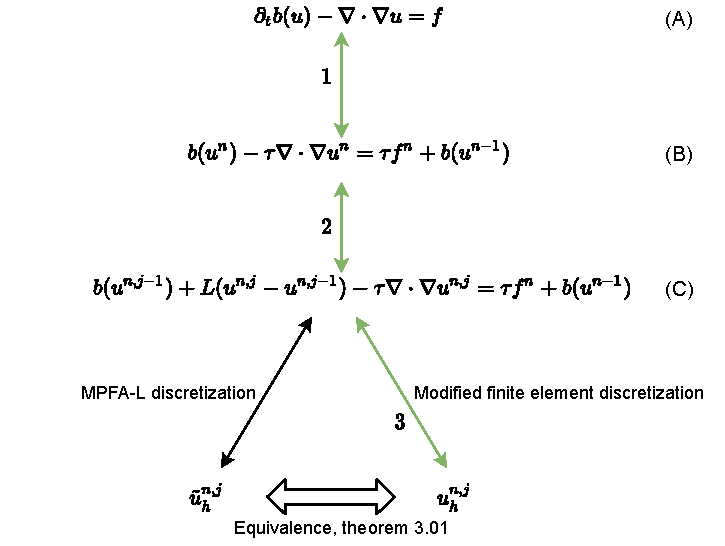
\includegraphics[width=0.8\textwidth]{convergence schema.pdf}
		\caption{}
		\label{fig:convergence schema}
	\end{figure}

	
	\begin{theorem}
		Richards' equation after Kirchhoff transform \eqref{eq:richards simple} discretized with backward Euler in time, L-scheme linearization and MPFA-L discretization in space \eqref{eq:linearized richards fvm} converges,
		\begin{equation}
			\tilde{u}_h^{n,j}\rightarrow u,
		\end{equation}
		as $j\rightarrow \infty$, $h\rightarrow 0$ and $\tau \rightarrow 0$.
	\end{theorem}
	\begin{proof}
		As the MPFA-L method and the modified finite element method are equivalent, we prove the convergence of our finite element solution, $u^{n,j}_h$.
		The proof will be done in three steps, see figure \ref{fig:convergence schema}.
		We have by the triangle inequality
		\begin{equation}
			\left \|u_h^{n,j}-u\right \|_1 \leq \left \|u_h^{n,j}-u^{n,j}\right \|_1 + \left \|u^{n,j}-u^n\right \|_1 + \left \|u^n - u \right \|_1.
		\end{equation}
		\begin{enumerate}
			\item The first term is the error of solving an elliptic problem
			\begin{equation}\label{eq:first ineq}
				u^{n,j}-\frac{\tau}{L} \nabla \cdot \nabla u^{n,j} = \frac{L u^{n,j-1} + \tau f^n - b(u^{n,j-1}) + u^{n-1}}{L}.
			\end{equation}
			By theorem \ref{th:convergence of elliptic} we have the error estimate
			\begin{equation}
				\left \|u_h^{n,j}-u^{n,j}\right \|_1  \leq C h (\left \| u^{n,j-1} \right \|_2 + \left \| \frac{L u^{n,j-1} + \tau f^n - b(u^{n,j-1}) + u^{n-1}}{L} \right \|_0 + \left \| g \right \|_{\frac{1}{2},\Gamma_N}).
			\end{equation}
		\item The second term, $\left \|u^{n,j}-u^n\right \|_1$,...
		\end{enumerate}
	\end{proof}
	
	
	\vspace{100pt}
	\textbf{Convergence of L-scheme for modified FEM}
	This is done (List, Radu, 2016,\cite{list2016study}) for the normal finite element method, but we do the proof here for our modified finite element method. 
	First we need assumptions on the parametrizations $\kappa $ and $\theta$:
	\begin{itemize}
		\item[\textbf{A 1}] The water content parametrization $\theta(\cdot)$ is monotonically increasing with $sup|\theta'| = L_{\theta}$ and Lipschitz continuos.
		\item[\textbf{A 2}] The permeability $\kappa$ is positive. 
	\end{itemize}
	\begin{theorem}
		Assume \textbf{A 1} and \textbf{A 2} above and that the constant L is chosen such that $L \geq L_{\theta}$. Then the L-scheme \eqref{eq:L-scheme-FEM} converges linearly. 
	\end{theorem}
	\begin{proof}
		Let as before $e^{n,j} = u^{n,j}-u^n$ be the iteration error.
		We start by subtracting \eqref{eq:richards_timedisc} from \eqref{eq:L-scheme-FEM} and obtain:
			\begin{equation}
			\begin{aligned}
				\left \langle \hat{I}_h \theta(u^{n,j-1}_h) - \hat{I}_h \theta(u^{n}_h),\hat{I}_h v_h \right \rangle_0 &+ L \left \langle \hat{I}_h e^{n,j}_h -  \hat{I}_h e^{n,j-1}_h,\hat{I}_h v_h \right \rangle_0 \\+ \tau \left \langle \kappa (\nabla u^{n,j}_h-\nabla u^{n}_h),\nabla v_h \right \rangle_0 &=0 
			\end{aligned}
		\end{equation}
		Now we test with $v_h=e^{n,j}$:
		\begin{equation}
			\begin{aligned}
				\left \langle \hat{I}_h \theta(u^{n,j-1}_h) - \hat{I}_h \theta(u^{n}_h),\hat{I}_h e^{n,j} \right \rangle_0 &+ L \left \langle \hat{I}_h e^{n,j}_h -  \hat{I}_h e^{n,j-1}_h,\hat{I}_h e^{n,j} \right \rangle_0 \\+ \tau \left \langle \kappa\nabla e^{n,j},\nabla e^{n,j} \right \rangle_0 &=0 
			\end{aligned}
		\end{equation}
		We use the identity $\left \langle x-y,x\right \rangle = \frac{1}{2}\left \| x \right \|^2 + \frac{1}{2}\left \| x-y \right \|^2 - \frac{1}{2} \left \| y \right \|^2$ and some algebraic manipulation to obtain:
		\begin{equation}
			\begin{gathered}
					\left \langle \hat{I}_h \theta(u^{n,j-1}_h) - \hat{I}_h \theta(u^{n}_h),\hat{I}_h e^{n,j-1} \right \rangle + 	\left \langle \hat{I}_h \theta(u^{n,j-1}_h) - \hat{I}_h \theta(u^{n}_h),\hat{I}_h e^{n,j} - \hat{I}_h e^{n,j-1}\right \rangle \\
					+\frac{L}{2}\left \| \hat{I} e^{n,j}\right \|^2 + \frac{L}{2}\left \| \hat{I} e^{n,j}-\hat{I}e^{n,j-1} \right \|^2 -\frac{L}{2}\left \| \hat{I} e^{n,j-1}\right \|^2 \\
				+ \tau \left \langle \kappa \nabla e^{n,j},\nabla e^{n,j} \right \rangle_0 =0 
			\end{gathered}
		\end{equation}
		Then we put some terms on the right hand side:
		\begin{equation}
			\begin{gathered}
				\left \langle \hat{I}_h \theta(u^{n,j-1}_h) - \hat{I}_h \theta(u^{n}_h),\hat{I}_h e^{n,j-1} \right \rangle +\frac{L}{2}\left \| \hat{I} e^{n,j}\right \|^2 	 \\
				 + \frac{L}{2}\left \| \hat{I} e^{n,j}-\hat{I}e^{n,j-1} \right \|^2 + 
				\tau \left \langle \kappa\nabla e^{n,j},\nabla e^{n,j} \right \rangle_0  = \\ - \left \langle \hat{I}_h \theta(u^{n,j-1}_h) - \hat{I}_h \theta(u^{n}_h),\hat{I}_h e^{n,j} - \hat{I}_h e^{n,j-1}\right \rangle+\frac{L}{2}\left \| \hat{I} e^{n,j-1}\right \|^2
			\end{gathered}
		\end{equation}
		Now we use the Cauchy-Schwarz inequality, and the monotonicity $\textbf{A 1}$ on the first term. Similarly we use Cauchy-Schwarz and $\textbf{A 2}$ on the second term. Finally we use Young's inequality on the first term on the right hand side.
		\begin{equation}
			\begin{gathered}
				\frac{1}{L_{\theta}}\left \| \hat{I}_h (\theta(u^{n,j-1}-\theta(u^{n}))) \right \|^2 + \frac{L}{2}\left \| \hat{I} e^{n,j}\right \|^2 \\
				+ \frac{L}{2}\left \| \hat{I} e^{n,j}-\hat{I}e^{n,j-1} \right \|^2 + \tau \kappa_m \left \| \nabla e^{n,j} \right \|^2 \\
				\leq \frac{1}{2L} \left \| \hat{I}_h(\theta (u^{n,j-1})-\theta (u^n) ) \right \|^2  + \frac{L}{2} \left \|\hat{I}_h( e^{n,j} - e^{n,j-1}) \right \|^2+\frac{L}{2}\left \| \hat{I} e^{n,j-1}\right \|^2
			\end{gathered}
		\end{equation} 
		Next we can use Poincaré inequality:
		\begin{equation}\label{eq:L-proof}
			\begin{gathered}
				\frac{L}{2}\left \| \hat{I}_h e^{n,j}\right\|^2 + \frac{\tau \kappa_m}{C_{\Omega}} \left \|e^{n,j} \right \|^2 \leq (\frac{1}{2L} - \frac{1}{L_{\theta}}) \left \| \hat{I}_h(\theta (u^{n,j-1}-\theta (u^n))) \right \|^2 +\frac{L}{2}\left \| \hat{I} e^{n,j-1}\right \|^2
			\end{gathered}
		\end{equation}
		Since $L_{\theta} \leq L$ we can remove the first term on the right side from the inequality. We can also use the lemma \ref{lemma:int_error} about the interpolation error:
		\begin{equation}
			\left \| \hat{I}_h e^{n,j} \right \|^2 = \left \| \hat{I}_h e^{n,j} - e^{n,j} + e^{n,j} \right \|^2 \leq (ch\left \| e^{n,j}\right \| + \left \| e^{n,j} \right \|)^2=(1+ch)^2\left \| e^{n,j} \right \|^2
		\end{equation}
		Now \eqref{eq:L-proof} becomes:
		\begin{equation}
			(\frac{L}{2}+\frac{\tau \kappa_m }{C_{\Omega}(1 + ch)^2})\left \| \hat{I}_h e^{n,j} \right \|^2 \leq \frac{L}{2} \left \| \hat{I}_h e^{n,j-1}\right \|^2
		\end{equation}
	\end{proof}
	
\end{document}